\begin{enumerate}[label=\thesubsection.\arabic*.,ref=\thesubsection.\theenumi]
\numberwithin{equation}{enumi}

\item Tabulate the transfer functions of a PID controller and its variants.
\\
\solution See Table \ref{table:ee18btech11021}.

\begin{table}[!ht]
\centering
\input{./tables/ee18btech11021.tex}
\caption{}
\label{table:ee18btech11021}
\end{table}


\item
For a unity Feedback system 
\begin{align}
    G(s) = \frac{K}{s(s+2)(s+4)(s+6)}
\end{align}
%
Design a PD Controller with $K_{v} = 2$ and Phase Margin 30\degree

\solution The gain after cascading the PD Controller with  G(s) is 
%
\begin{align}
    G_{c}(s) = \frac{K_{p}(1 + T_{d}s)K}{s(s+2)(s+4)(s+6)}
\label{eq:ee18btech11021}
\end{align}
%
Choosing  $K_{p} = 1$ in \label{eq:ee18btech11021},
%
\begin{align}
    K_{v} &= \lim_{s \to 0} sG_{c}(s) = 2
\\
    \implies K &= 96
\end{align}

For Phase Margin 30\degree, at Gain Crossover Frequency $\omega$,
%
\begin{multline}
    \tan^{-1}\brak{T_{d}\omega} - \tan^{-1}\brak{\frac{\omega}{2}} - \tan^{-1}\brak{\frac{\omega}{4}}
\\
-    \tan^{-1}\brak{\frac{\omega}{6}} = -60 \degree
\end{multline}

\begin{align}
    \abs{G_{1}\brak{\j\omega}} = \frac{96\sqrt{T_{d}^2\omega^2 + 1}}{\omega\sqrt{(\omega^2+4)(\omega^2 + 16)(\omega^2 + 36)}} = 1
\end{align}

By Hit and Trial, one of the best combinations is
\begin{align}
    \omega = 4
\end{align}
\begin{align}
    T_{d} = 1.884
\end{align}
We get a Phase Margin of 30.31\degree

\item
Verify using a Python Plot

\solution The following code plots Fig. \ref{fig:ee18btech11021_pd}

\begin{lstlisting}
codes/ee18btech11021/EE18BTECH11021_3.py
\end{lstlisting}

\begin{figure}[!ht]
\centering
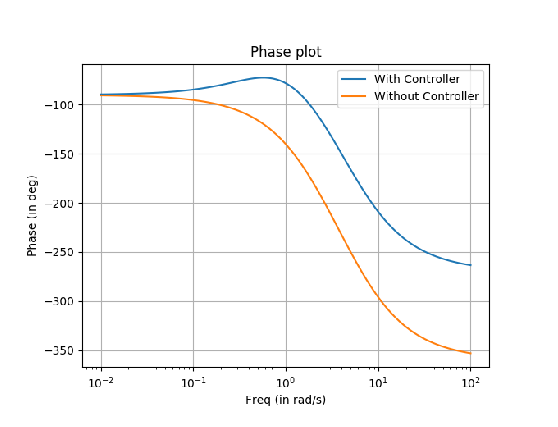
\includegraphics[width=\columnwidth]{./figs/ee18btech11021/EE18BTECH11021_PD.eps}
\caption{}
\label{fig:ee18btech11021_pd}
\end{figure}

\item
Design a PI Controller with $K_{v} = \infty$ and Phase Margin 30\degree

\solution From Table \ref{table:ee18btech11021}, the open loop gain in this case is

\begin{align}
    G_{1}(s) = \frac{K_{p}\brak{1 +  \frac{1}{T_{i}s}}K}{s(s+2)(s+4)(s+6)}
\end{align}

Choose $K_{p}K = 96$. Then
\begin{align}
    G_{1}(s) = \frac{96(T_{i}s + 1)}{T_{i}s^2(s+2)(s+4)(s+6)}
\end{align}

For Phase Margin 30\degree, at Gain Crossover Frequency $\omega$

\begin{multline}
    \tan^{-1}(T_{i}\omega) - \tan^{-1}\brak{\frac{\omega}{2}} - \tan^{-1}\brak{\frac{\omega}{4}}
\\
-    \tan^{-1}\brak{\frac{\omega}{6}} = 30
\end{multline}
and
\begin{align}
    \abs{G_{1}\brak{\j\omega}} = \frac{96\sqrt{T_{i}^2\omega^2 + 1}}{T_{i}^2\omega^2\sqrt{(\omega^2+4)(\omega^2 + 16)(\omega^2 + 36)}} = 1
\end{align}

By Hit and Trial, one of the best combinations is
\begin{align}
    \omega &= 0.75
\\
    T_{i} &= 2.713
\end{align}
We get a Phase Margin of 25.53\degree

\item
Verify using a Python Plot

\solution The following code plots Fig. \ref{fig:ee18btech11021_pi}.

\begin{lstlisting}
codes/ee18btech11021/EE18BTECH11021_4.py
\end{lstlisting}

\begin{figure}[!ht]
\centering
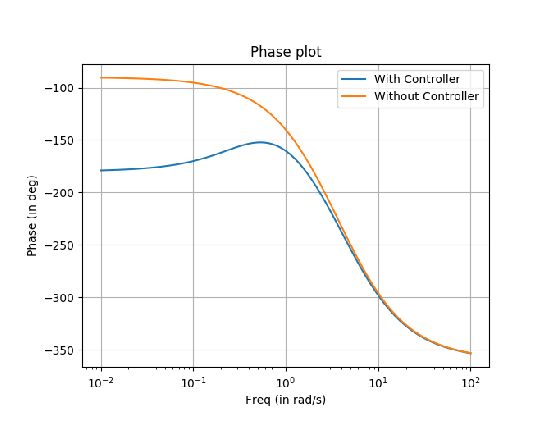
\includegraphics[width=\columnwidth]{./figs/ee18btech11021/EE18BTECH11021_PI.eps}
\caption{}
\label{fig:ee18btech11021_pi}
\end{figure}

\item
Design a PID Controller with $K_{v} = \infty$ and Phase Margin 30\degree

\solution

\begin{align}
    G_{1}(s) = \frac{K_{p}\brak{1 + T_{d}s + \frac{1}{T_{i}s}}K}{s(s+2)(s+4)(s+6)}
\end{align}

Choose $K_{p}K = 96$.  The open loop gain is
\begin{align}
    G_{1}(s) = \frac{96(T_{i}T_{d}s^2 + T_{i}s +  1)}{T_{i}s^2(s+2)(s+4)(s+6)}
\end{align}

For Phase Margin 30\degree, at Gain Crossover Frequency $\omega$,

\begin{multline}
    \tan^{-1}\brak{\frac{T_{i}\omega}{1-T{i}T_{d}w^2}} - \tan^{-1}\brak{\frac{\omega}{2}} - \tan^{-1}\brak{\frac{\omega}{4}}
\\
-    \tan^{-1}\brak{\frac{\omega}{6}} = 30
\end{multline}

\begin{multline}
    \abs{G_{1}\brak{\j\omega}} 
\\
= \frac{96\sqrt{(1-T{i}T_{d}\omega^2)^2 + T_{i}^2}}{T_{i}^2\omega^2\sqrt{(\omega^2+4)(\omega^2 + 16)(\omega^2 + 36)}} = 1
\end{multline}

By Hit and Trial, one of the best combinations is
\begin{align}
    \omega &= 1
\\
    T_{i} &= 1.738
\\
    T_{d} &= 0.4
\end{align}
We get a Phase Margin of 30\degree

\item
Verify using a Python Plot

\solution  The following code plots Fig. \ref{fig:EE18BTECH11021_PID}

\begin{lstlisting}
codes/ee18btech11021/EE18BTECH11021_5.py
\end{lstlisting}

\begin{figure}[!ht]
\centering
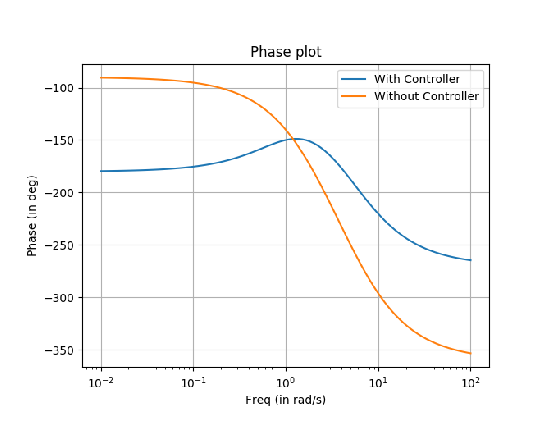
\includegraphics[width=\columnwidth]{./figs/ee18btech11021/EE18BTECH11021_PID.eps}
\caption{}
\label{fig:EE18BTECH11021_PID}
\end{figure}
\end{enumerate}
